\documentclass[12pt]{report}

\usepackage[utf8]{inputenc}
\usepackage[T1]{fontenc}
\usepackage[english]{babel}
\usepackage{setspace}
\usepackage{geometry}
\usepackage{graphicx}
\usepackage{float}
\usepackage{hyperref}


\geometry{a4paper, margin=1in}


\onehalfspacing

\begin{document}


\begin{titlepage}
    \centering
    

    {\Large \textbf{Titanic: Machine Learning from Disaster} \par}
    \vspace{0.5cm}
    {\large \textbf{System Analysis Project} \par}
    \vspace{3cm}
    
    {\large 
    Julián Carvajal Garnica \\ 
    20242020024 \\[0.5cm]
    Andrés Mauricio Cepeda Villanueva \\
    20242020010 \\[0.5cm]
    Jhonatan David Moreno Barragán \\
    20201020094 \\[0.5cm]
    Andrés Camilo Ramos Rojas \\
    20242020005
    }
    
    \vfill
    

    School of Engineering, Universidad Distrital Francisco José de Caldas \\
    System Analysis Course \\
    Teacher: Carlos Andrés Sierra \\
    Bogotá D.C. \\
    2025
    
\end{titlepage}


\chapter*{Part 2 of the System Analysis Project}

\section*{1. Review of Workshop \#1 Findings}

The analytical work from Workshop \#1 provided a comprehensive understanding of the Titanic competition as a dynamic and interdependent system. Rather than treating it as a simple prediction problem, the study highlighted structural dependencies, sensitivity points, and chaotic behaviors that influence model performance and reliability.

\subsection*{System Overview and Core Elements}

The system’s main objective is to predict passenger survival using multiple features — such as class, sex, age, and family relations — extracted from \texttt{train.csv}, \texttt{test.csv}, and \texttt{gender\_submission.csv}. Each dataset interacts with the others through defined roles in the machine learning pipeline: data ingestion, preprocessing, model training, and evaluation within Kaggle’s controlled environment.

\subsection*{Data Characteristics and Constraints}

Several structural constraints were identified in the datasets:
\begin{itemize}
    \item Missing or incomplete values in \texttt{Age}, \texttt{Cabin}, and \texttt{Embarked}
    \item Class imbalance biasing model learning
    \item Limited dataset size (approximately 1,300 samples), increasing risk of overfitting
\end{itemize}

\subsection*{Sensitivity and Complexity}

The system displays high sensitivity to key predictors (\texttt{Sex}, \texttt{Pclass}, \texttt{Age}). Removing or misprocessing them decreases accuracy. Nonlinear relationships such as \texttt{Sex} $\times$ \texttt{Age} and \texttt{Pclass} $\times$ \texttt{Fare} create complex interactions requiring feature engineering and regularization.

\subsection*{Chaos and Randomness}

Even structured datasets like Titanic’s contain unpredictability. Passengers with similar profiles sometimes had opposite outcomes due to hidden variables. Family-related variables (\texttt{SibSp}, \texttt{Parch}) introduce feedback loops, reflecting emergent nonlinear behavior—an echo of chaos theory in data.

\subsection*{Implications for System Design}

These findings guide the system design foundations: modularity, robustness, and controlled randomness. Each stage—from data ingestion to model evaluation—must minimize instability and maximize reproducibility.


\section*{2. System Requirements Definition}

\subsection*{Functional Requirements}

\begin{table}[H]
\centering
\begin{tabular}{|p{1cm}|p{4cm}|p{9cm}|}
\hline
\textbf{ID} & \textbf{Requirement} & \textbf{Description} \\ \hline
FR-1 & Data Ingestion Module & Load and validate input datasets (\texttt{train.csv}, \texttt{test.csv}, and \texttt{gender\_submission.csv}). \\ \hline
FR-2 & Preprocessing and Cleaning & Handle missing or null values in variables such as \texttt{Age}, \texttt{Cabin}, and \texttt{Embarked}. \\ \hline
FR-3 & Feature Engineering & Apply transformations (e.g., one-hot encoding for categorical variables). \\ \hline
FR-4 & Model Training & Train a supervised learning model (e.g., Random Forest) to predict \texttt{Survived}. \\ \hline
FR-5 & Evaluation and Metrics & Compute model accuracy and generate submission file. \\ \hline
FR-6 & Submission Output & Export predictions to \texttt{submission.csv} following Kaggle’s structure. \\ \hline
\end{tabular}
\caption{Functional Requirements}
\end{table}

\subsection*{Non-Functional Requirements}

\begin{table}[H]
\centering
\begin{tabular}{|p{1cm}|p{4cm}|p{9cm}|}
\hline
\textbf{ID} & \textbf{Requirement} & \textbf{Description} \\ \hline
NFR-1 & Performance & Process datasets (1,300 records) in less than 5 seconds. \\ \hline
NFR-2 & Scalability & Allow easy addition of features without refactoring. \\ \hline
NFR-3 & Reproducibility & Use fixed random seeds and documented dependencies. \\ \hline
NFR-4 & Maintainability & Modular architecture separating stages. \\ \hline
NFR-5 & Usability & Provide clear workflow and outputs. \\ \hline
NFR-6 & Reliability & Handle corrupted input files gracefully. \\ \hline
\end{tabular}
\caption{Non-Functional Requirements}
\end{table}

\subsection*{Sensitivity-Driven Requirements}

\begin{itemize}
    \item \textbf{SR-1 – Controlled Randomness:} Use fixed random seeds in training.
    \item \textbf{SR-2 – Robust Feature Selection:} Include key predictors (\texttt{Sex}, \texttt{Pclass}, \texttt{Age}).
    \item \textbf{SR-3 – Missing Data Resilience:} Apply imputation strategies.
    \item \textbf{SR-4 – Monitoring and Feedback:} Log performance metrics to detect anomalies.
\end{itemize}

\subsection*{User-Centric Requirements}

\begin{itemize}
    \item \textbf{UR-1 – Simplicity:} Execute workflow in one notebook sequence.
    \item \textbf{UR-2 – Interpretability:} Provide explainable feature relationships.
    \item \textbf{UR-3 – Security:} Prevent exposure of private Kaggle data.
\end{itemize}

\noindent
These requirements translate the \textit{Workshop 1} insights into engineering goals that ensure an \textbf{accurate, reproducible, and resilient} predictive system.


\section*{3. High-Level Architecture}
\begin{figure}[H]
    \centering
    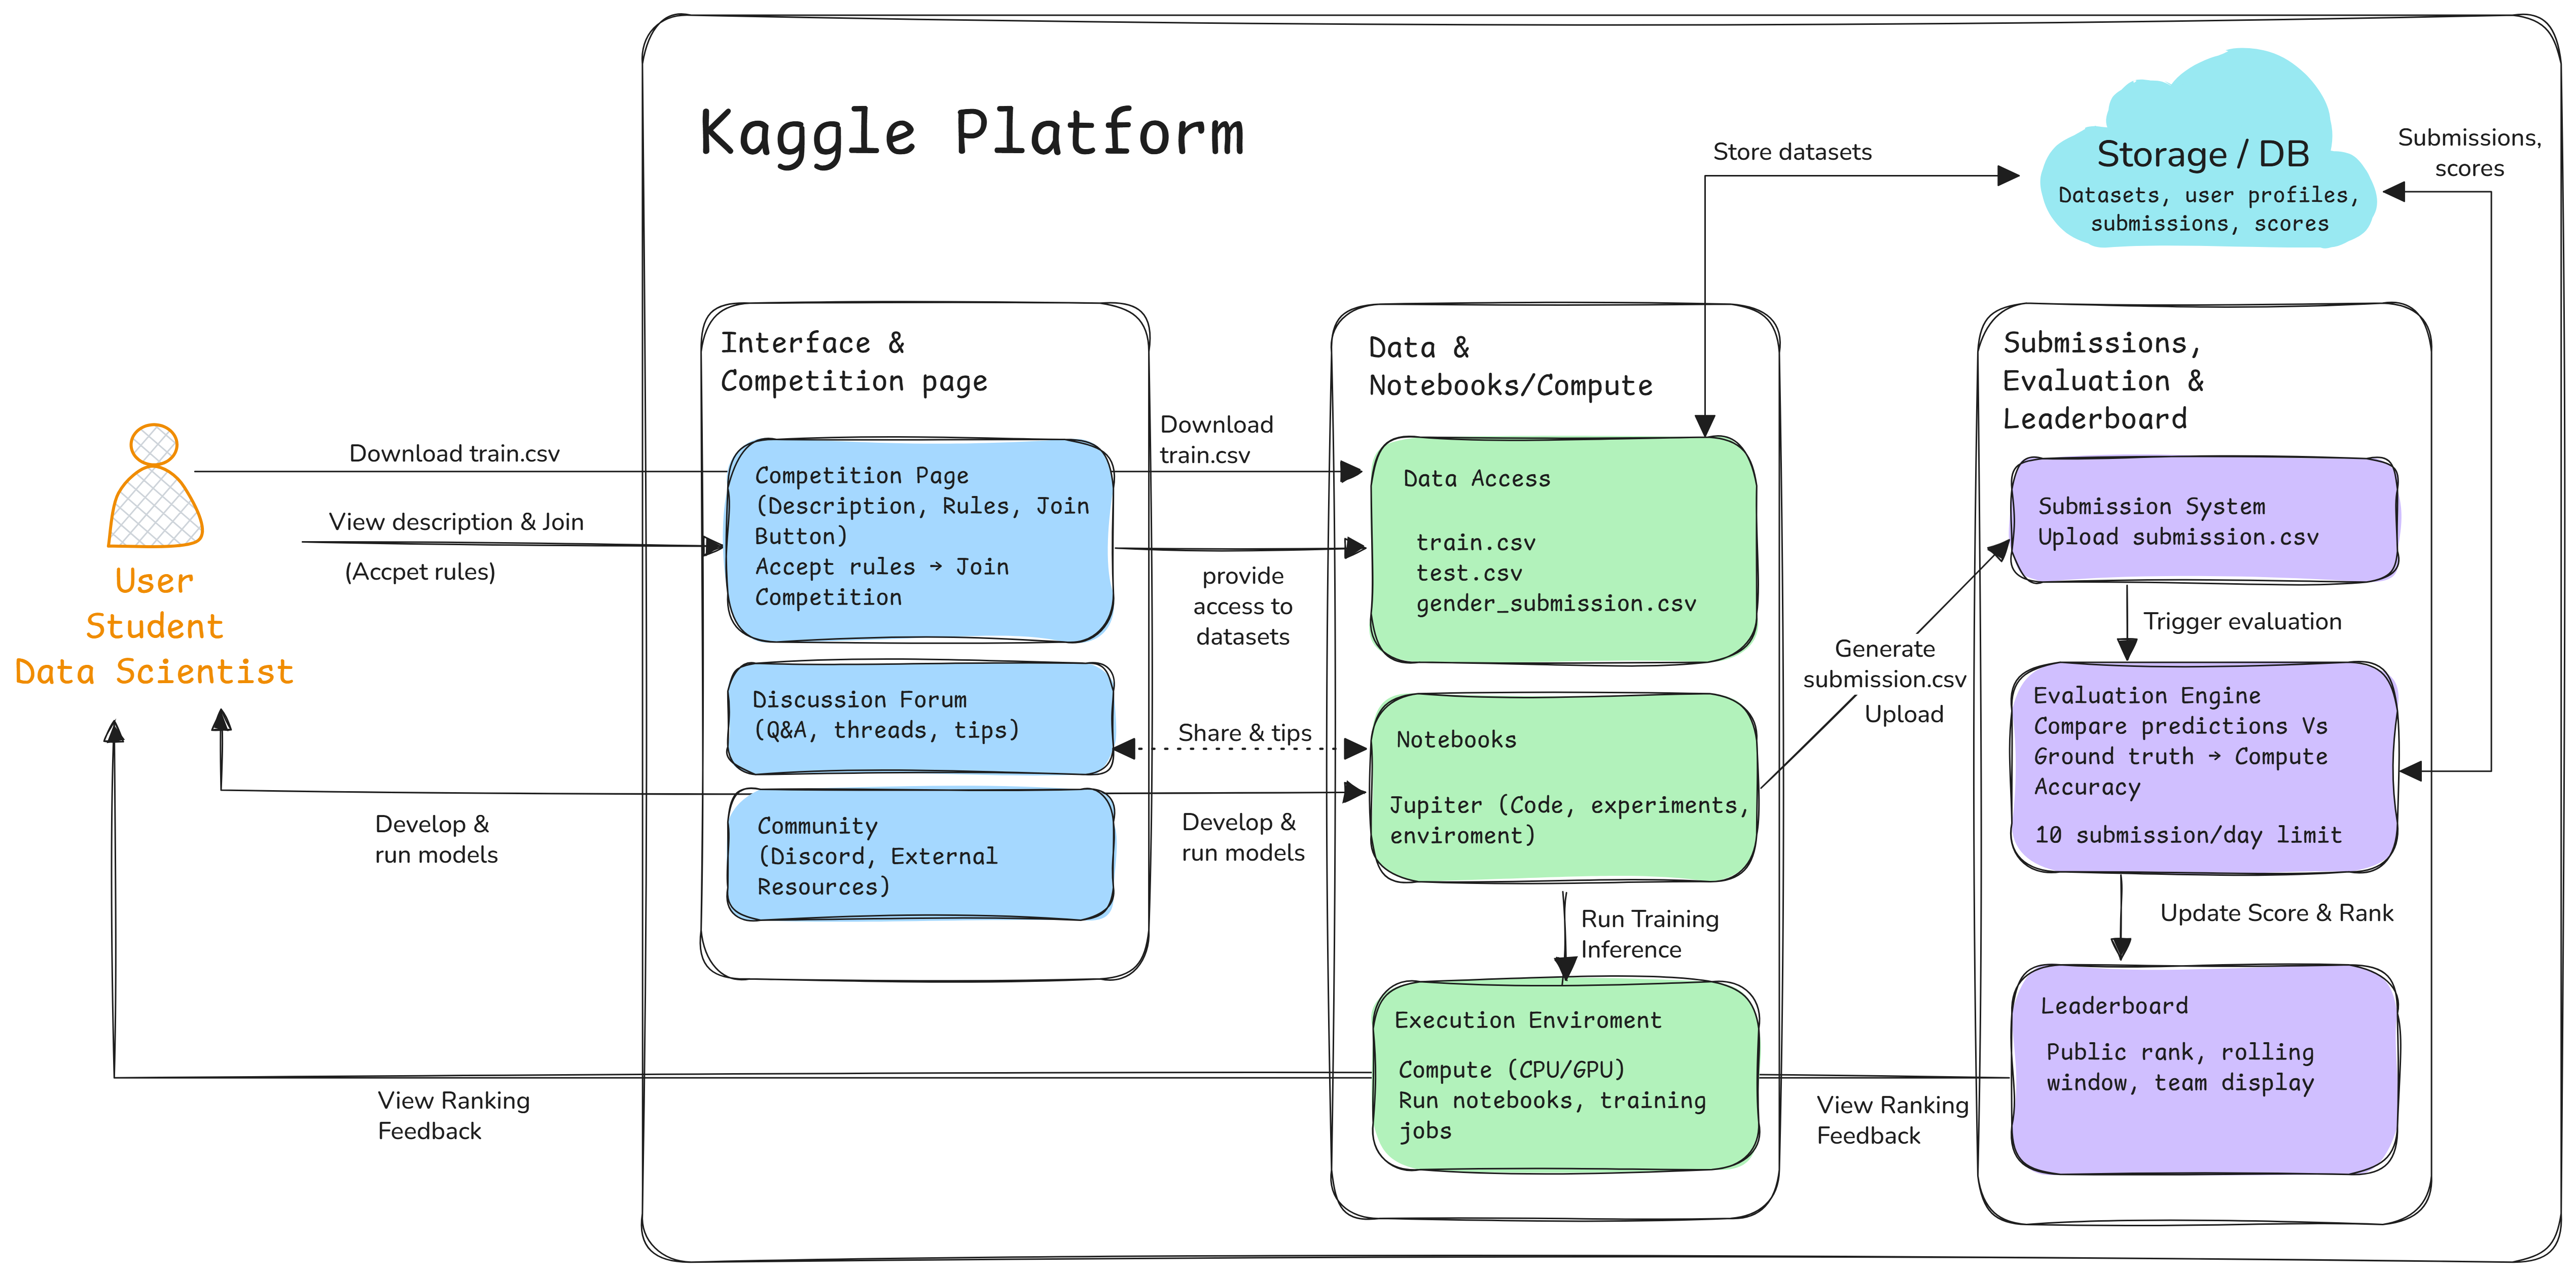
\includegraphics[width=\linewidth]{Figure1.png}
    \caption{Architecture of the Kaggle competition environment.}
    \label{fig:system-architecture}
\end{figure}

\noindent
\textbf{Figure \ref{fig:system-architecture}} illustrates the architecture of the Kaggle competition environment. Competitors access the competition page, download datasets, train models in notebooks, and submit predictions for evaluation. The system computes accuracy, updates leaderboards, and integrates community interaction via forums and repositories.
\begin{itemize}
    \item \textbf{User:} The user will be an ordinary person regardless of their occupation; in reality, they only need to have an interest in the world of systems analysis, with access to practically the entire system except for certain interactions that will be carried out internally by the system.
    \item \textbf{Interface \& competition page:} This module allows the user to interact directly with the competency environment, meaning that they are allowed to access the competency and view all the necessary information to understand the environment. Additionally, there are community environments that allow users to ask questions about the competencies.
    \item \textbf{Data \& Notebooks/Compute:} This module allows the user to dive into the competition, accessing the data that will be used, the testing environment, and resources such as the notebooks provided by Kaggle for a better understanding of the competition.
    \item \textbf{Storage/DB:} This module is not directly accessible to the user but interacts with them indirectly by sending information that will be stored for later viewing, as in the leaderboard or in the different saved files.
    \item \textbf{Submissions, Evolution \& Leaderboard:} This module allows the user to finalize their attempt in the competition by submitting the presented model to improve the prediction algorithm, as well as assigning a ranking by comparing it with the other submitted solutions.
\end{itemize}
\section*{4. Addressing Sensitivity and Chaos} 
It is inevitable to deal with random factors. In the case of the Titanic, we can imagine damaged gates, someone being far from the escape routes, falling awkwardly into the water and being unable to stay afloat. There are many factors that can have an impact. Likewise, we find nonlinear relationships which will be somewhat random since there is nothing that can describe them accurately, as a linear function would. For all the above reasons, a robust and well-divided system is proposed in which it is possible to identify the implications of the elements among themselves more clearly, aiming for a better approximation of who has the capacity to survive and who does not. This is evidenced through the tests provided by the competition, where cases of people with very similar characteristics but opposite outcomes are found, although we also understand that it could be due to a lack of consideration of important variables.\\
It would be extremely positive to start taking into account those values that we find to be random for a more exhaustive review and to find out which other variables could affect both sensitivity, as well as an unexpected variable or others.
\end{document}
